\documentclass[]{article}
\usepackage{lmodern}
\usepackage{amssymb,amsmath}
\usepackage{ifxetex,ifluatex}
\usepackage{fixltx2e} % provides \textsubscript
\ifnum 0\ifxetex 1\fi\ifluatex 1\fi=0 % if pdftex
  \usepackage[T1]{fontenc}
  \usepackage[utf8]{inputenc}
\else % if luatex or xelatex
  \ifxetex
    \usepackage{mathspec}
  \else
    \usepackage{fontspec}
  \fi
  \defaultfontfeatures{Ligatures=TeX,Scale=MatchLowercase}
\fi
% use upquote if available, for straight quotes in verbatim environments
\IfFileExists{upquote.sty}{\usepackage{upquote}}{}
% use microtype if available
\IfFileExists{microtype.sty}{%
\usepackage{microtype}
\UseMicrotypeSet[protrusion]{basicmath} % disable protrusion for tt fonts
}{}
\usepackage[margin=1in]{geometry}
\usepackage{hyperref}
\hypersetup{unicode=true,
            pdftitle={Epigenomic prediction of cardiovascular disease risk and interactions with traditional risk metrics},
            pdfborder={0 0 0},
            breaklinks=true}
\urlstyle{same}  % don't use monospace font for urls
\usepackage{graphicx,grffile}
\makeatletter
\def\maxwidth{\ifdim\Gin@nat@width>\linewidth\linewidth\else\Gin@nat@width\fi}
\def\maxheight{\ifdim\Gin@nat@height>\textheight\textheight\else\Gin@nat@height\fi}
\makeatother
% Scale images if necessary, so that they will not overflow the page
% margins by default, and it is still possible to overwrite the defaults
% using explicit options in \includegraphics[width, height, ...]{}
\setkeys{Gin}{width=\maxwidth,height=\maxheight,keepaspectratio}
\IfFileExists{parskip.sty}{%
\usepackage{parskip}
}{% else
\setlength{\parindent}{0pt}
\setlength{\parskip}{6pt plus 2pt minus 1pt}
}
\setlength{\emergencystretch}{3em}  % prevent overfull lines
\providecommand{\tightlist}{%
  \setlength{\itemsep}{0pt}\setlength{\parskip}{0pt}}
\setcounter{secnumdepth}{0}
% Redefines (sub)paragraphs to behave more like sections
\ifx\paragraph\undefined\else
\let\oldparagraph\paragraph
\renewcommand{\paragraph}[1]{\oldparagraph{#1}\mbox{}}
\fi
\ifx\subparagraph\undefined\else
\let\oldsubparagraph\subparagraph
\renewcommand{\subparagraph}[1]{\oldsubparagraph{#1}\mbox{}}
\fi

%%% Use protect on footnotes to avoid problems with footnotes in titles
\let\rmarkdownfootnote\footnote%
\def\footnote{\protect\rmarkdownfootnote}

%%% Change title format to be more compact
\usepackage{titling}

% Create subtitle command for use in maketitle
\providecommand{\subtitle}[1]{
  \posttitle{
    \begin{center}\large#1\end{center}
    }
}

\setlength{\droptitle}{-2em}

  \title{Epigenomic prediction of cardiovascular disease risk and interactions
with traditional risk metrics}
    \pretitle{\vspace{\droptitle}\centering\huge}
  \posttitle{\par}
    \author{}
    \preauthor{}\postauthor{}
    \date{}
    \predate{}\postdate{}
  
\usepackage{booktabs}
\usepackage{longtable}
\usepackage{array}
\usepackage{multirow}
\usepackage{wrapfig}
\usepackage{float}
\usepackage{colortbl}
\usepackage{pdflscape}
\usepackage{tabu}
\usepackage{threeparttable}
\usepackage{threeparttablex}
\usepackage[normalem]{ulem}
\usepackage{makecell}
\usepackage{xcolor}

\usepackage{booktabs}
\usepackage{longtable}
\usepackage{array}
\usepackage{multirow}
\usepackage{wrapfig}
\usepackage{float}
\usepackage{pdflscape}
\usepackage{tabu}
\usepackage{threeparttable}
\usepackage{threeparttablex}
\usepackage[normalem]{ulem}
\usepackage{makecell}

\begin{document}
\maketitle

Kenneth Westerman\textsuperscript{1}, Alba
Fernández-Sanlés\textsuperscript{2,3}, Prasad Patil\textsuperscript{4},
Paola Sebastiani\textsuperscript{4}, Paul Jacques\textsuperscript{1},
John M. Starr \textsuperscript{5,6}, Ian Deary\textsuperscript{5,6},
Qing Liu\textsuperscript{7}, Simin Liu\textsuperscript{7}, Roberto
Elosua\textsuperscript{2,8,9}, Dawn L. DeMeo\textsuperscript{10}, José
M. Ordovás\textsuperscript{1,11,12}

\textsuperscript{1}JM-USDA Human Nutrition Research Center on Aging at
Tufts University, Boston, MA, USA, \textsuperscript{2}Cardiovascular
Epidemiology and Genetics Research Group, REGICOR Study group, IMIM
(Hospital del Mar Medical Research Institute), Barcelona, Catalonia,
Spain, \textsuperscript{3}Pompeu Fabra University (UPF), Barcelona,
Catalonia, Spain, \textsuperscript{4}Department of Biostatistics, Boston
University School of Public Health, Boston, MA, USA,
\textsuperscript{5}Department of Psychology, University of Edinburgh,
Edinburgh, UK, \textsuperscript{6}Centre for Cognitive Ageing and
Cognitive Epidemiology, University of Edinburgh, Edinburgh, UK,
\textsuperscript{7}Department of Epidemiology, Brown University School
of Public Health, Providence, RI, USA, \textsuperscript{8} CIBER
Cardiovascular Diseases (CIBERCV), Spain, \textsuperscript{9} Medicine
Department, Medical School, University of Vic-Central University of
Catalonia (UVic-UCC), Vic, Catalonia, Spain,
\textsuperscript{10}Channing Division of Network Medicine, Department of
Medicine, Brigham and Women's Hospital, Boston, MA, USA,
\textsuperscript{11}IMDEA Alimentación, CEI, UAM, Madrid, Spain,
\textsuperscript{12}Centro Nacional de Investigaciones Cardiovasculares
(CNIC), Madrid, Spain

\hypertarget{abstract}{%
\section{Abstract}\label{abstract}}

Epigenome-wide association studies for cardiometabolic risk factors have
discovered multiple loci associated with incident cardiovascular disease
(CVD). However, few studies have sought to directly optimize a predictor
of CVD risk. Furthermore, it is challenging to train multivariate models
across multiple studies in the presence of study- or batch effects.
Here, we analyzed existing DNA methylation data collected using the
Illumina HumanMethylation450 microarray to create a predictor of CVD
risk across three cohorts: Women's Health Initiative, Framingham Heart
Study Offspring Cohort, and Lothian Birth Cohorts. We trained Cox
proportional hazards-based elastic net regressions for incident CVD
separately in each cohort, and used a recently-introduced cross-study
learning approach to integrate these individual predictions into an
ensemble predictor. The methylation-based risk score (MRS) predicted CVD
time-to-event in a held-out fraction of the Framingham dataset (HR per
SD = 1.28, p = 2e-3) and predicted myocardial infarction status in the
independent REGICOR dataset (OR per SD = 2.14, p = 9e-7). These
associations remained after adjustment for traditional cardiovascular
risk factors and were similar to those from elastic net models trained
on a directly merged dataset. Additionally, we investigated interactions
between the MRS and both genetic and biochemical CVD risk, showing
preliminary evidence of an enhanced predictive power in those with less
traditional risk factor elevation. This investigation provides
proof-of-concept for a genome-wide, CVD-specific epigenomic risk score
and suggests that the DNA methylation data may enable the discovery of
high-risk individuals that would be missed by alternative risk metrics.

\hypertarget{introduction}{%
\section{Introduction}\label{introduction}}

DNA methylation is an important epigenetic pathway through which genetic
variants and environmental exposures impact disease
risk\textsuperscript{1,2}. Methylation at specific
cytosine-phosphate-guanine (CpG) sites has been associated with disease
in epigenome-wide association studies, even showing associations in
blood as a convenient but non-target tissue such as for type 2
diabetes\textsuperscript{3}. Methylation-based risk scores allow
genome-wide aggregation of epigenetic information, similarly to the more
established genetic risk scores, and allow for the use of models with
arbitrary complexity. These risk scores are often developed initially by
using methylation as a proxy for disease risk factors, such as body mass
index (BMI)\textsuperscript{4} and general aging-related
morbidity\textsuperscript{5}. Alternatively, given sufficient sample
size, epigenetic associations with disease risk can be modeled
directly\textsuperscript{6}.

Associations between DNA methylation and cardiovascular disease (CVD)
have been explored in many different cohorts and using diverse
approaches. Cross-sectional associations have been found across multiple
relevant tissues, namely blood, aorta, and other vascular
tissues\textsuperscript{7}. Some investigations aimed at cardiovascular
risk factors have discovered CpGs predictive of CVD
development\textsuperscript{8,9}, while Mendelian randomization
approaches have suggested causality of at least some of these CpG-risk
factor associations\textsuperscript{10}. A few studies directly modeling
incident CVD as a primary outcome have either been conducted using only
global (not locus-specific) methylation levels\textsuperscript{11}, or
have found limited additional predictive power in the presence of known
risk factors\textsuperscript{12}. A recent large-scale meta-analysis
found multiple CpG sites predictive of incident coronary heart disease,
but focused on univariate approaches\textsuperscript{13}. We have
previously investigated methylation regions and modules associating with
incident CVD, generating mechanistic insights but without aggregating
these results into a direct predictor of risk\textsuperscript{14}.
Additionally, it is unclear how the CVD risk tracked by DNA methylation
is redundant with or complementary to existing risk metrics, including
genetic scores\textsuperscript{15} and those based on traditional
cardiovascular risk factors (e.g.~the Framingham Risk Score for
generalized CVD)\textsuperscript{16}.

Combining signal across population-scale cohorts can increase sample
size while attenuating the effect of study-specific biases and
confounding factors, but can be prone to emergent sources of confounding
from ``batch'' effects or other systematic biases in methylation data
across cohorts. This is especially problematic when there is notable
class imbalance (i.e.~different outcome frequencies) across
cohorts\textsuperscript{17}. The most common method for dealing with
this heterogeneity is meta-analysis, but standard meta-analysis
approaches are restricted to univariate (one CpG site at a time) models.
Other approaches include batch effect correction on the input dataset
(e.g.~ComBat\textsuperscript{18}), direct adjustment for batch/study in
linear models, or adjustment for derived variables intended to capture
technical biases (e.g.~surrogate variable analysis\textsuperscript{19}),
but these approaches can often lead to over- or under-estimates of true
biological effects\textsuperscript{17}. An alternative approach
described recently, cross-study learning, instead trains an ensemble
predictor consisting of one or multiple models per
cohort\textsuperscript{20}. This strategy allows the use of arbitrarily
complex models while avoiding technical confounding from direct
combination of the datasets.

In order to develop an improved DNA methylation-based cardiovascular
risk predictor using multiple training cohorts, we used a cross-study
learning method to develop an ensemble of penalized time-to-event
regression risk models. The resulting composite risk score performed
well in a held-out data subset, predicting survival even in the presence
of traditional risk factors, and showing similar performance to models
trained on naively merged datasets. External validation was achieved in
a case-control for prevalent myocardial infarction (MI). Further,
interactions were assessed between the composite methylation-based risk
score and other risk predictors, finding a potentially enhanced
prediction in those with low Framingham Risk Scores.

\hypertarget{methods}{%
\section{Methods}\label{methods}}

\hypertarget{study-participants-and-phenotype-collection}{%
\subsection{Study participants and phenotype
collection}\label{study-participants-and-phenotype-collection}}

Phenotypes (demographic, anthropometric, biochemical, and clinical), DNA
methylation data, and imputed genotypes were available either from
publicly available controlled-access databases or upon request from the
cohorts. Cohort-specific details are provided in Supplementary methods.
Blood-based biochemical markers (total cholesterol, LDL-cholesterol,
HDL-cholesterol, triglycerides, fasting glucose, high-sensitivity
C-reactive protein, and systolic blood pressure) were log10-transformed
for all analyses. In the Lothian Birth Cohort 1936, LDL was estimated
from total cholesterol and triglycerides using the Friedewald equation.
Diabetes was defined as either use of diabetes medication or a measured
fasting blood glucose level of \textgreater{}125 mg/dL. Median
imputation was used to fill missing values for diabetes, medication use,
and smoking status (thus assuming no diabetes, no medication use, and no
smoking where these values were missing). Analysis of these datasets was
approved by the Tufts University Health Sciences Institutional Review
Board (protocol 12592), and all subjects gave informed consent.

\hypertarget{dna-methylation-data-processing}{%
\subsection{DNA methylation data
processing}\label{dna-methylation-data-processing}}

DNA methylation data for all initial cohorts (WHI, FHS, and LBC) were
collected using the Illumina HumanMethylation450 microarray
platform\textsuperscript{21} and downloaded as raw intensity files.
Standard preprocessing steps were performed for each cohort, including
sample-wise and probe-wise filters, background correction, and probe
type normalization. After quality control and filtering steps, 390597
CpG sites were shared between the 3 datasets, formatted as beta values
(ratio of methylated signal to total microarray signal). Preprocessing
details are described in the Supplementary Methods.

\hypertarget{cvd-risk-prediction-modeling}{%
\subsection{CVD risk prediction
modeling}\label{cvd-risk-prediction-modeling}}

Study-specific CVD risk prediction models were trained using penalized
Cox proportional hazards regressions with the elastic net penalty. CVD
events were defined as above, and times were right-censored based on the
most recent exam available in each cohort. The elastic alpha parameter
was set at 0.05, based on prior observations of good performance on
Illumina methylation microarray datasets\textsuperscript{22}, and the
penalty parameter \(\lambda\) was optimized through 5-fold
cross-validation. For each model, only the most variable 100,000 CpGs
according to median absolute deviation (\textasciitilde{}25\% of all
available sites shared across platforms) were included in order to
decrease the computational burden and ensure that the selected CpGs
would have meaningful interindividual variation.

The cross-study learner (CSL) was constructed as an ensemble of
study-specific regression models. Predictions from each single-study
learner (SSL) were combined using the ``stacking''
approach\textsuperscript{20}, implemented as follows. First, predictions
from each SSL to both itself and the other training datasets were
combined into a design matrix (with dimensions \(N_{total}\) x \# SSLs).
This formed the input to an additional penalized Cox regression (ridge
regression with \(\lambda\) optimized through 5-fold CV and coefficients
restricted to be non-negative) of all training studies at once.
Coefficients from this regression, corresponding to input study-specific
SSLs, were normalized to sum to one to produce the CSL weights. For
prediction in new datasets, SSL predictions were each standardized to
mean zero and unit variance before calculating their weighted sum (using
the ``stacking'' weights) as the final CSL score.

A series of approaches for combining information across cohorts were
tested as alternatives to the CSL. The naive ``combined'' approach
consisted of simply aggregating observations from all training sets into
a single dataset and training an elastic net regression as described
above while adjusting for study as a fixed effect. The ComBat method
trained across all studies as with the ``combined'' approach, but
included an empirical Bayes-based preprocessing step to directly adjust
the dataset for study differences while preserving variation along the
``axis'' of incident CVD events\textsuperscript{18}.

MRS evaluation in FHS was performed using Cox proportional hazards
models, with a series of models adjusting for covariates including
demographics, anthropometrics, biochemical values, and cell subtype
estimates. Robust standard errors were used to account for family
structure as has been suggested for clustered data\textsuperscript{23}
and used for epigenetic risk models in FHS\textsuperscript{24}. The
proportional hazards assumption was confirmed (p \textgreater{} 0.05)
using the \emph{cox.zph} R function. To compare risk scores generated
using different models (combined and ComBat-preprocessed) to the CSL,
Cox regressions adjusting for the ``basic'' covariate set were used to
evaluate the CSL MRS alone, the CSL MRS plus the combined MRS, and the
CSL MRS plus the ComBat-preprocessed MRS in the held-out FHS-UM dataset.
Likelihood ratio tests were then used to compare each of the two-MRS
models to that CSL-only model, with the resulting p-values indicating
whether either of these alternative scores provided additional
predictive benefit. MRS evaluation in the REGICOR case-control used
logistic regression models, adjusting for the same sets of covariates
where possible, though traditional biochemical risk factors were only
available in discrete low vs.~high categories.

The biology underlying the CSL model was evaluated through a series of
enrichment tests using the component CpG loci and annotated genes. Gene
ontology-based enrichment analysis of each cohort-specific model was
performed using the gometh function from the \emph{missMethyl} package
for R\textsuperscript{25}. This procedure uses gene annotations for CpGs
from the HumanMethylation450 microarray annotation from Illumina (v1.0
B2). Enrichment analysis is then performed for each gene ontology
category using Wallenius' noncentral hypergeometric distribution to
account for inconsistent representation of CpG sites across genes. The
overall merged set of CpGs included in the final CSL model was then
tested for enrichment in transcription factor binding sites using HOMER
tool\textsuperscript{26}. CpG loci (with respect to genome build hg19)
were provided as inputs, with 200 base-pair windows and repeat-masked
sequences.

\hypertarget{genomic-risk-score-calculation}{%
\subsection{Genomic risk score
calculation}\label{genomic-risk-score-calculation}}

Imputed genotype data for WHI were retrieved from dbGaP (accession:
phs000746.v2.p3. Variants were filtered for imputation R-squared
\textgreater{} 0.3, and annotated with rsIDs, loci, and allelic
information using the 1000 Genomes Phase 3 download from dbSNP (download
date: April 13, 2018). Weights for the genetic risk score calculation
(6,630,151 variants) were based on the genome-wide CVD score developed
by Khera et al\textsuperscript{15}. We note that these scores were
developed only for populations of European descent, and thus are not
optimized for the mixed-ancestry WHI population. GRS were then
calculated as the weighted sum of allelic dosages, normalized by the
number of relevant SNPs available. Genotype data processing and GRS
calculation were performed using PLINK 2.0.

\hypertarget{risk-score-interaction-analysis}{%
\subsection{Risk score interaction
analysis}\label{risk-score-interaction-analysis}}

Interaction analysis was performed using similar Cox regression models
to those above, adjusting for the ``basic'' set of covariates and using
robust standard error estimates. To facilitate visual comparisons,
main-effect regressions for the MRS were fitted within risk strata
defined by the FRS or GRS separately in each dataset. To obtain overall
interaction effect estimates, an interaction between MRS and either FRS
or GRS was introduced into a combined regression including all datasets,
while allowing stratified baseline hazards (strata() argument to the
coxph function). We note that main effects in the interaction analysis
are biased upwards since the regression datasets were used for training
the MRS. Regressions assessing the GRS excluded non-white participants
to match the ancestry used to develop the CVD score\textsuperscript{15}.

For quasi-replication of these associations in the REGICOR dataset,
stratified logistic regressions were used to discriminate MI cases from
controls using the MRS, while adjusting for estimated cell count
fractions as well as two SVA components (as in the main REGICOR models).
In the absence of continuous values for blood pressure and lipids, an
empirical risk function was generated by first performing a logistic
regression on the following cardiovascular risk factors: age, sex,
estimated cell count fractions, BMI, diabetes, smoking status,
hyperlipidemia (binary), and hypertension (binary), along with two SVA
components. Predicted risks based on this model were then used to
stratify subjects into four risk groups by evenly splitting the range of
predicted risks into four segments (thus resulting in strata based on
raw risk, rather than percentiles).

\hypertarget{results}{%
\section{Results}\label{results}}

\hypertarget{cross-study-learner-model-development}{%
\subsection{Cross-study learner model
development}\label{cross-study-learner-model-development}}

Epigenomic model development was performed in three cohorts, including
the Women's Health Initiative (WHI), Framingham Heart Study Offspring
Cohort (FHS), and Lothian Birth Cohort 1936 (LBC). The FHS dataset was
divided into two functionally separate groups (FHS-JHU and FHS-UM) based
on differences in subject selection and geographic location of
laboratory methylation analysis (see Methods). Further population
details can be found in Table 1.

\begin{table}[t]

\caption{\label{tab:pop-description}Baseline parameters of the populations used for model development}
\centering
\begin{threeparttable}
\begin{tabular}{lllll}
\toprule
Study/Subset & WHI & FHS-JHU & LBC & FHS-UM\\
Sample size & 2023 & 484 & 818 & 2103\\
Age & 65 (59-70) & 71 (64-77) & 69 (68-70) & 64 (59-71)\\
Sex (female) & 2023 (100\%) & 145 (30\%) & 406 (50\%) & 1270 (60\%)\\
\addlinespace[0em]
\multicolumn{5}{l}{Ancestry}\\
\hspace{1em}\% European & 959 (47\%) & 484 (100\%) & 818 (100\%) & 2103 (100\%)\\
\hspace{1em}\% African American & 651 (32\%) & 0 (0\%) & 0 (0\%) & 0 (0\%)\\
\hspace{1em}\% Hispanic & 413 (20\%) & 0 (0\%) & 0 (0\%) & 0 (0\%)\\
Body mass index & 29.1 (25.5-33.3) & 28.2 (25.5-31.3) & 27.5 (24.9-30.3) & 27.4 (24.3-31)\\
LDL cholesterol & 150 (126-175) & 88 (73-107) & 118 (89.5-150.3) & 107 (87-128)\\
HDL cholesterol & 51 (43-60) & 49 (40-60) & 56.1 (47.2-68.3) & 56 (45.8-69)\\
Triglycerides & 127 (92-177) & 101.5 (75-141.2) & 128.4 (97.4-171.2) & 102 (73-142)\\
Fasting glucose & 96 (88.6-108) & 106 (97-116) & Unavailable & 100 (94-109)\\
Systolic blood pressure & 131 (120-143) & 130 (117-143) & 148.7 (137-161.3) & 126 (116-138)\\
\addlinespace[0em]
\multicolumn{5}{l}{\# CVD events}\\
\hspace{1em}Prior only & 0 & 127 & 70 & 112\\
\hspace{1em}Incident only & 1009 & 67 & 133 & 146\\
\hspace{1em}Prior and incident & 0 & 58 & 164 & 34\\
\bottomrule
\end{tabular}
\begin{tablenotes}
\item * Continuous values shown as: median (interquartile range)
\item WHI = Women's Health Initiative, FHS-JHU = Framingham Heart Study Offspring Cohort (Johns Hopkins University subset), LBC = Lothian Birth Cohorts 1936, FHS-UM = Framingham Heart Study Offspring Cohort (University of Minnesota subset)
\end{tablenotes}
\end{threeparttable}
\end{table}

Fig. 1 outlines the computational workflow. Briefly, a cross-study
learning (CSL) model was developed by training time-to-event elastic net
regressions on three of the datasets, while holding out the FHS-UM
subset for evaluation. Next, a model trained on all four datasets was
subject to external replication in the REGICOR study. CSL model CpGs
were characterized as to their potential biological function, and model
performance was assessed across strata of alternative cardiovascular
risk metrics.

The initial predictor was developed by training individual penalized Cox
proportional hazards regression models (single-study learners, or SSLs)
in each of the three training cohorts (WHI, FHS-JHU, and LBC).
Predictions from these models were aggregated through a ``stacking''
method, in which the outcomes and model predictions from each of the
individual datasets are combined, and a regression is used to assign
weights to each of the model predictions (see Methods). This procedure
led to FHS-JHU dropping out of the ensemble model, with weights for this
initial predictor as follows: 0.57 (WHI), 0.0 (FHS-JHU), and 0.43 (LBC).
This result means that FHS-JHU did not generalize (i.e.~to WHI and LBC)
as well as the other two components models.

\hypertarget{assessment-in-held-out-fhs-subset}{%
\subsection{Assessment in held-out FHS
subset}\label{assessment-in-held-out-fhs-subset}}

\begin{table}[t]

\caption{\label{tab:fhs-holdout}MRS performance in held-out FHS subset}
\centering
\begin{threeparttable}
\begin{tabular}{lrl}
\toprule
Model & HR per s.d. MRS\textsuperscript{a} & P-value\\
\midrule
Unadjusted\textsuperscript{1} & 1.58 & 5.4e-10\\
Basic\textsuperscript{2} & 1.28 & 2.0e-03\\
Plus risk factors\textsuperscript{3} & 1.29 & 2.7e-03\\
FRS only\textsuperscript{4} & 1.36 & 2.0e-05\\
\bottomrule
\end{tabular}
\begin{tablenotes}
\item[a] Estimated hazard ratio per standard deviation of the methylation-based risk score
\item[1] No covariates
\item[2] Adjusted for age, sex, and estimated cell type fractions
\item[3] Additionally adjusted for BMI, LDL, HDL, SBP, diabetes status, and current smoking
\item[4] Adjusted for Framingham Risk Score only
\end{tablenotes}
\end{threeparttable}
\end{table}

Stacking of the three initial predictors resulted in model weights of
0.57, 0, and 0.43 for WHI, FHS-JHU, and LBC, respectively (i.e.~the
FHS-JHU sub-model did not ultimately contribute to the initial ensemble
model). The resulting ensemble predictor was evaluated using robust Cox
proportional hazards models in FHS-UM, showing strong associations with
incident CVD in an unadjusted model (HR=1.58, 95\% CI: 1.37-1.83), which
was attenuated partially through adjustment for standard covariates
(age, sex, and estimated cell type fractions; HR=1.28, 95\% CI:
1.10-1.50) as well as CVD risk factors (HR=1.29, 95\% CI: 1.09-1.51).
Results for the unadjusted model and three sensitivity models are shown
in Table 2. These results were robust to sensitivity analyses excluding
all individuals who experienced prior CVD events (Supp. Table S1), and
produced similar results when incident event status was analyzed as a
binary outcome using logistic regression (p = 3.3e-4).

Results from comparison of CSL performance to models trained on combined
datasets (either naive combination or including preprocessing using
ComBat) are shown in Supp. Fig. S1. The ComBat-preprocessed model had
modestly higher hazard ratios in FHS-UM, while relative differences with
the combined model depended on the covariates included. However,
likelihood ratio tests using the Basic model covariates (age, sex, and
cell type fraction-adjusted) did not reveal a strong added predictive
benefit of either the combined (p = 0.58) or ComBat (p = 0.08) risk
scores over that using only the CSL.

\hypertarget{final-csl-model-characterization}{%
\subsection{Final CSL model
characterization}\label{final-csl-model-characterization}}

The stacking regression in the final CSL model gave the most weight to
WHI (0.48) and LBC (0.38), while retaining nonzero weights for FHS-JHU
(0.06) and FHS-UM (0.08). This result indicates that the WHI and
LBC-trained models were better able to generalize to the other cohorts
than vice versa. There was very little overlap of specific CpG sites
across cohort-specific models, with a maximum of 13 CpGs shared between
two models (WHI and FHS-UM) and no CpGs shared between three or more
models (Fig. 3a). Despite this lack of site-specific overlap, there was
broad agreement for three of the four component SSL models at the level
of enriched biological processes, with all except FHS-JHU enriched most
strongly for proximity to genes involved in homophilic cell adhesion
(Fig. 3b). MRS component CpGs tended to be found in similar genomic loci
to the overall set of variable CpGs, and were enriched in gene bodies
and depleted in CpG islands compared to the full microarray CpG set.
However, MRS CpGs did show a modest enrichment in and around CpG islands
compared to the set of variable CpGs (Fig. 3d). To seek more clarity as
to potential biological mechanisms represented by the MRS, the HOMER
tool was used to calculate enrichment of transcription factor (TF)
binding motifs in the MRS component CpG sites. Using the union of all
individual SSL CpG sites as input, no strong enrichments were found (all
q-values \textgreater{}0.5).

To better understand the stability of the risk score over time,
intraclass correlation coefficients (ICCs) were calculated for two sets
of grouped samples: 26 technical replicates from FHS and approximately
1000 longitudinal samples (across 3 visits, or about 6 years total) from
LBC (Supp. Table S2). The technical replicates showed an ICC of 0.85,
while the longitudinal samples showed an ICC of 0.68. As would be
expected, the ICC for samples closer in time (Waves 1 \& 2; ICC = 0.69)
were higher than that for samples more distant in time (Waves 1 \& 3;
ICC = 0.61). Based on the observation of imperfect stability of the MRS
over time as well as the partial attenuation in predictive power after
adjustment for age, its component CpGs (the 1305-element union of all
CpGs in any of the four individual SSL models) were examined for overlap
with established epigenetic age metrics. While no enrichment was seen
for the original cross-tissue DNAm age from Horvath\textsuperscript{27},
strong enrichment was seen for the morbidity-directed
PhenoAge\textsuperscript{5} (9 of 513 CpGs; p=2.3e-5) and especially the
blood-specific aging marker from Hannum et al.\textsuperscript{28} (13
of 71 CpGs; p=5.9e-21). We note that these overlaps do not constitute a
major fraction of either CpG set, but are nonetheless highly
statistically significant. The PhenoAge metric is based on some known
cardiovascular risk factors (e.g.~C-reactive protein) and is known to
associate with CVD, but is not trained in any of the cohorts included
here.

\hypertarget{discrimination-in-myocardial-infarction-case-control}{%
\subsection{Discrimination in myocardial infarction
case-control}\label{discrimination-in-myocardial-infarction-case-control}}

\begin{table}[t]

\caption{\label{tab:regicor}Results from replication in REGICOR MI case-control}
\centering
\begin{threeparttable}
\begin{tabular}{llll}
\toprule
Model & ComBat & Combined & CSL\\
\midrule
Unadjusted & 1.79 [1.39-2.31] & 1.86 [1.45-2.38] & 1.83 [1.41-2.37]\\
Basic & 2.16 [1.58-2.93] & 2.12 [1.57-2.87] & 2.14 [1.58-2.89]\\
Plus risk factors & 1.76 [1.22-2.54] & 1.66 [1.15-2.4] & 1.61 [1.11-2.34]\\
\bottomrule
\end{tabular}
\begin{tablenotes}
\item * Results are presented as: OR per s.d. MRS [95\% CI]
\item * Model covariates as in Table 2
\item * All models above are adjusted for two surrogate variable analysis (SVA) components.
\end{tablenotes}
\end{threeparttable}
\end{table}

As one form of replication, the MRS was investigated for its
discriminative performance in a nested case-control for prior myocardial
infarction in the REGICOR cohort (Table 3; cohort description in Supp.
Table S3). Though this dataset contained prevalent (rather than
incident) events, its matching of sex and age allowed an evaluation free
of potential confounding by these factors. The MRS was able to
discriminate cases and controls in both unadjusted (odds ratio = 1.79, p
= 6.33e-6) and, to a lesser degree, risk factor-adjusted models (odds
ratio = 1.61, p = 0.019). Given the relatively large confidence
intervals, there was no meaningful difference in odds ratios across
modeling strategies (Combined, ComBat, and CSL) for any of the
adjustment models.

\hypertarget{interactions-with-alternate-risk-metrics}{%
\subsection{Interactions with alternate risk
metrics}\label{interactions-with-alternate-risk-metrics}}

To understand how the present risk score interacts with other
established CVD risk metrics, the performance of the MRS was
re-evaluated after stratifying individuals by risk scores reflecting
either demographic and biochemical features (Framingham Risk Score), or
genetic variants (based on Khera et al.~2018). First, the marginal
effects of these risk scores were confirmed in each population. The
Framingham Risk Score (FRS) was strongly predictive in WHI and FHS,
while surprisingly showing no association with CVD incidence in LBC
(Supp. Table S4). The genetic score was evaluated in WHI, demonstrating
a moderate association with CVD (odds ratio per standard deviation =
1.28, p = 1.1e-6).

In Cox models using baseline hazards stratified by study and performed
using the final four-study MRS, it appeared that the MRS was more
effective in those in lower ``traditional'' risk strata (according to
the FRS; Fig. 4). As a sensitivity analysis, the cohorts were fully
stratified into separate models, in which this pattern was visually
clear in WHI and FHS-JHU (Supp. Fig. S2). The pattern did not appear in
LBC, although we note that the Framingham Risk Score also did not show a
``main effect'' for predicting incident CVD in this cohort. A similar
pattern appeared with respect to genetic risk in WHI (European ancestry
participants only based on the formulation of the relevant risk score),
in which maximum MRS performance was achieved in the lowest alternative
risk stratum. Supplementing these visual comparisons, combined Cox
regressions across all cohorts (allowing for different baseline hazards
across studies) showed a strong MRS-FRS interaction effect (7\%
reduction in HR for the MRS per 10\% increase in FRS; p = 8.27e-05),
while that for the MRS-GRS interaction did not reach nominal statistical
significance (2\% reduction in HR for the MRS per standard deviation
increase in GRS; p = 0.719).

To explore the clinical potential of these interactions further, we
returned to the initial MRS (trained in 3 datasets with FHS-UM held
out). The FHS-UM dataset was filtered to include only participants with
lower CVD risk based on the FRS (\textless{}10\% estimated 10-year
risk). Within this lower-risk subset, participants in the upper MRS
quintile had more than double the risk of the remainder of the
participants: 7\% (12/176) versus 3\% (19/701).

FRS could not be calculated in the REGICOR dataset, as not all risk
factors were available as continuous values. However, stratified models
replicated the observation of greater MRS discrimination in the lowest
alternative risk stratum. An empirical risk function was generated
through logistic regression of MI status on cardiovascular risk factors
(age, sex, BMI, diabetes, smoking status, hyperlipidemia (binary), and
hypertension). Predicted MI risk using this model was used to stratify
subjects into four risk groups, with MRS odds ratios (per standard
deviation) of 4.49 in the lowest-risk group versus 1.20 in the
highest-risk group. More detailed results from these analyses are shown
in Supp. Table S5.

\hypertarget{discussion}{%
\section{Discussion}\label{discussion}}

Epigenetic signatures of cardiometabolic diseases and aging in general
are being actively explored as biomarkers of disease risk that are
potentially modifiable and reveal underlying biological mechanisms.
Here, in a novel application of a cross-study ensembling method, we
introduce a DNA methylation-based score specific to cardiovascular
disease risk. The model performs similarly to one trained on a direct
combination of the component datasets, and may be most strongly
predictive in individuals predicted to be at lower risk based on
traditional risk factors.

We opted to use cross-study learning to train our risk model based on
the expectation that differences across cohorts (e.g.~demographic,
behavioral) may contribute to heterogeneity in both the marginal
distribution of the CpG features and the conditional distribution of the
CVD outcome. Under these conditions, the generalizability of a
single-study predictor is often obscured or
overstated\textsuperscript{29,30}. The performance of the CSL model was
similar to that of models trained on the merged cohorts with or without
batch adjustment via ComBat. This suggests that the assumptions made by
these direct combination strategies (i.e.~that the heterogeneity
structure can be captured by variation in the marginal effects of each
CpG site) are met. In practice, this underlying structure is unknown,
and we highlight that the CSL was able to produce similar gains in
predictive accuracy without making specific assumptions.

In assessing the stability of the MRS, we observed reasonable
reproducibility between technical replicates (ICC=0.85). ICCs for LBC
subjects over time were somewhat lower (ICC=0.68), which is to be
expected due to not only changes in environment, but also the known
epigenetic evolution with age that we observed to be enriched in the
components of our score. Furthermore, this value is at the upper end of
the range of single-CpG repeatability measurements over time calculated
in the combined Lothian Birth Cohorts (1921 and
1936)\textsuperscript{31}. These ICC values suggest an imperfect but
usable reproducibility of the MRS, and an aggregate marker that is
fairly robust considering the low replicability that has been observed
for individual sites in technical replicates (general median ICC of 0.3
and mode of 0.75 in a ``high reliability'' cluster)\textsuperscript{32}.

The enrichment of the MRS component CpGs for proximity to genes related
to cell-cell adhesion (in all subsets except FHS-JHU) is indicative of
the underlying biological mechanisms. As we have previously observed in
the WHI and FHS cohorts, it appears that immune activation is central to
the prognostic information contained in leukocyte DNA
methylation\textsuperscript{14}. For example, epigenetic processes have
been shown to be involved in the activation and increased adhesion of
monocytes in response to environmental insults and metabolic stress,
though these have been explored primarily in relation to histone
modifications\textsuperscript{33}. Our results provide preliminary
support for an attractive model in which a methylation-based score could
act as a monitor of cumulative stress in leukocytes and their
corresponding activation towards a more atherogenic state.

Existing epigenetic scores have shown varying strength in predicting
incident cardiovascular disease. An early investigation examined
blood-based methylation in LINE-1 elements, finding strong associations
of global hypomethylation with prevalent and incident ischemic heart
disease global (LINE-1), though additional reports showed opposite
associations of methylation at repetitive elements with
CVD\textsuperscript{34}. Guarrera et al.~developed a biomarker for MI
based on global LINE-1 and ZBTB12 gene methylation that provided a
modest net reclassification index improvement (0.23-0.47) compared to
traditional risk factors only. Multiple epigenetic aging metrics, though
not developed specifically for CVD, have been shown to predict incident
CHD, including PhenoAge (odds ratios from 1.02 to 1.08) and GrimAge
(hazard ratio = 1.07, adjusted for age and technical
factors)\textsuperscript{5,24}. While these associations are
statistically significant, they do not represent clinically meaningful
improvements in discrimination. Our observed hazard ratio of 1.28 (Basic
model in the held-out FHS-UM dataset) indicates that this MRS may be
closer to clinical relevance. We note that our component CpG sites
overlap strongly with those of these established epigenetic metrics
including PhenoAge, suggesting that it captures some of the same
biological patterns. However, the mechanistic significance of the
specific methylation signals captured by these aging-related metrics,
whether as markers of epigenetic regulation breakdown or the work of an
``epigenetic maintenance system'', is still
unclear\textsuperscript{27,35}.

In examining the potential clinical utility of an novel risk score for
CVD, it is important to understand to what extent it is redundant with
or complementary to existing risk metrics. This type of cross-metric
analysis can be clinically relevant, as demonstrated for example in a
recent investigation exploring the interaction between genetic and
lifestyle-based risk prediction for dementia\textsuperscript{36}. Here,
we saw a pattern of improved epigenetic risk prediction in individuals
whose cardiovascular risk based on traditional metrics (here, the
Framingham Risk Score) was low. This pattern replicated in the REGICOR
dataset (though FRS could not be directly calculated), with improved MRS
discrimination in lower-risk subjects based on an empirical risk
function. While these associations are preliminary, they suggest that an
epigenetic risk score could help identify higher-risk individuals who
otherwise would not have been detected by other metrics. While we did
not identify any robust patterns of differential MRS performance in
strata based on a genetic cardiovascular risk score, there may have been
lower power to detect any such patterns from the outset given the modest
discriminatory performance of the GRS in WHI.

Multiple limitations should be acknowledged. While lymphocytes are known
to be important in CVD pathogenesis, there is likely additional
biological signal in other CVD-relevant tissues not examined here.
Additionally, the present definition of CVD was chosen to balance
specificity of CVD subtypes with sample size, but this balance could be
altered to focus on more specific disease subtypes (e.g.~myocardial
infarction) or a broader definition of CVD (e.g.~including heart
failure). Finally, while the REGICOR dataset provided an important age-
and sex-matched case-control setting for replication of the MRS, this
work would benefit from future replication in an independent cohort
enabling assessment of incident disease.

In sum, we have developed an epigenetic risk score for cardiovascular
disease that provides additional predictive power beyond existing risk
measures, and may show improved performance in populations otherwise
designated as low-risk. Furthermore, we have shown a novel application
of a cross-cohort ensembling method that may provide significant value
to future investigations in genomic epidemiology.

\hypertarget{acknowledgements}{%
\section{Acknowledgements}\label{acknowledgements}}

We thank all LBC1936 study participants and research team members. The
LBC1936 is supported by Age UK (Disconnected Mind program) and the
Medical Research Council (MR/M01311/1). Methylation typing in LBC1936
was supported by Centre for Cognitive Ageing and Cognitive Epidemiology
(Pilot Fund award), Age UK, The Wellcome Trust Institutional Strategic
Support Fund, The University of Edinburgh, and The University of
Queensland. LBC1936 work was conducted in the Centre for Cognitive
Ageing and Cognitive Epidemiology, which is supported by the Medical
Research Council and Biotechnology and Biological Sciences Research
Council (MR/K026992/1), and which supported IJD.

\hypertarget{references}{%
\section{References}\label{references}}

\hypertarget{refs}{}
\leavevmode\hypertarget{ref-Bonder2016}{}%
1. Bonder MJ, Luijk R, Zhernakova DV, Moed M, Deelen P, Vermaat M, et
al. Disease variants alter transcription factor levels and methylation
of their binding sites. \emph{Nature Genetics}. 2016;49:131--138.

\leavevmode\hypertarget{ref-Tobi2018}{}%
2. Tobi EW, Slieker RC, Luijk R, Dekkers KF, Stein AD, Xu KM, et al. DNA
methylation as a mediator of the association between prenatal adversity
and risk factors for metabolic disease in adulthood. \emph{Science
Advances}. 2018;4:eaao4364.

\leavevmode\hypertarget{ref-Bacos2016}{}%
3. Bacos K, Gillberg L, Volkov P, Olsson AH, Hansen T, Pedersen O, et
al. Blood-based biomarkers of age-associated epigenetic changes in human
islets associate with insulin secretion and diabetes. \emph{Nature
Communications}. 2016;7:11089.

\leavevmode\hypertarget{ref-Wahl2017}{}%
4. Wahl S, Drong A, Lehne B, Loh M, Scott WR, Kunze S, et al.
Epigenome-wide association study of body mass index and the adverse
outcomes of adiposity. \emph{Nature}. 2017;541:81--86.

\leavevmode\hypertarget{ref-Levine2018}{}%
5. Levine ME, Lu AT, Quach A, Chen BH, Assimes TL, Bandinelli S, et al.
An epigenetic biomarker of aging for lifespan and healthspan.
\emph{Aging}. 2018;10:573--591.

\leavevmode\hypertarget{ref-Hao2017}{}%
6. Hao X, Luo H, Krawczyk M, Wei W, Wang W, Wang J, et al. DNA
methylation markers for diagnosis and prognosis of common cancers.
\emph{Proceedings of the National Academy of Sciences}.
2017;114:7414--7419.

\leavevmode\hypertarget{ref-Fernandez-Sanles2017}{}%
7. Fernández-Sanlés A, Sayols-Baixeras S, Subirana I, Degano IR, Elosua
R. Association between DNA methylation and coronary heart disease or
other atherosclerotic events: A systematic review. 2017;263:325--333.

\leavevmode\hypertarget{ref-Hedman2017}{}%
8. Hedman ÅK, Mendelson MM, Marioni RE, Gustafsson S, Joehanes R, Irvin
MR, et al. Epigenetic Patterns in Blood Associated With Lipid Traits
Predict Incident Coronary Heart Disease Events and Are Enriched for
Results From Genome-Wide Association Studies. \emph{Circulation:
Cardiovascular Genetics}. 2017;10:e001487.

\leavevmode\hypertarget{ref-Aslibekyan2018}{}%
9. Aslibekyan S, Agha G, Colicino E, Do AN, Lahti J, Ligthart S, et al.
Association of Methylation Signals With Incident Coronary Heart Disease
in an Epigenome-Wide Assessment of Circulating Tumor Necrosis Factor
\(\alpha\). \emph{JAMA Cardiology}. 2018;3:463--472.

\leavevmode\hypertarget{ref-Richardson2017}{}%
10. Richardson TG, Zheng J, Davey Smith G, Timpson NJ, Gaunt TR, Relton
CL, et al. Mendelian Randomization Analysis Identifies CpG Sites as
Putative Mediators for Genetic Influences on Cardiovascular Disease
Risk. \emph{American Journal of Human Genetics}. 2017;101:590--602.

\leavevmode\hypertarget{ref-Baccarelli2010}{}%
11. Baccarelli A, Wright R, Bollati V, Litonjua A, Zanobetti A,
Tarantini L, et al. Ischemic heart disease and stroke in relation to
blood DNA methylation. \emph{Epidemiology}. 2010;21:819--828.

\leavevmode\hypertarget{ref-Guarrera2015}{}%
12. Guarrera S, Fiorito G, Onland-Moret NC, Russo A, Agnoli C, Allione
A, et al. Gene-specific DNA methylation profiles and LINE-1
hypomethylation are associated with myocardial infarction risk.
\emph{Clinical Epigenetics}. 2015;7:133.

\leavevmode\hypertarget{ref-Agha2019}{}%
13. Agha G, Mendelson MM, Ward-Caviness CK, Joehanes R, Huan T, Gondalia
R, et al. Blood Leukocyte DNA Methylation Predicts Risk of Future
Myocardial Infarction and Coronary Heart Disease. \emph{Circulation}.
2019;140:645--657.

\leavevmode\hypertarget{ref-Westerman2018}{}%
14. Westerman K, Sebastiani P, Jacques P, Liu S, DeMeo D, Ordovás JM.
DNA methylation modules associate with incident cardiovascular disease
and cumulative risk factor exposure. \emph{bioRxiv}. 2018;471722.

\leavevmode\hypertarget{ref-Khera2018}{}%
15. Khera AV, Chaffin M, Aragam KG, Haas ME, Roselli C, Choi SH, et al.
Genome-wide polygenic scores for common diseases identify individuals
with risk equivalent to monogenic mutations. \emph{Nature Genetics}.
2018;50:1219--1224.

\leavevmode\hypertarget{ref-DAgostino2008}{}%
16. D'Agostino RB, Vasan RS, Pencina MJ, Wolf PA, Cobain M, Massaro JM,
et al. General cardiovascular risk profile for use in primary care: The
Framingham heart study. \emph{Circulation}. 2008;117:743--753.

\leavevmode\hypertarget{ref-Goh2017}{}%
17. Goh WWB, Wang W, Wong L. Why Batch Effects Matter in Omics Data, and
How to Avoid Them. 2017;35:498--507.

\leavevmode\hypertarget{ref-Johnson2007}{}%
18. Johnson WE, Li C, Rabinovic A. Adjusting batch effects in microarray
expression data using empirical Bayes methods. \emph{Biostatistics}.
2007;8:118--127.

\leavevmode\hypertarget{ref-Leek2007}{}%
19. Leek JT, Storey JD. Capturing Heterogeneity in Gene Expression
Studies by Surrogate Variable Analysis. \emph{PLoS Genetics}.
2007;3:e161.

\leavevmode\hypertarget{ref-Patil2018}{}%
20. Patil P, Parmigiani G. Training replicable predictors in multiple
studies. \emph{Proceedings of the National Academy of Sciences}.
2018;115:2578--2583.

\leavevmode\hypertarget{ref-Bibikova2011}{}%
21. Bibikova M, Barnes B, Tsan C, Ho V, Klotzle B, Le JM, et al. High
density DNA methylation array with single CpG site resolution.
\emph{Genomics}. 2011;98:288--295.

\leavevmode\hypertarget{ref-Zhuang2012}{}%
22. Zhuang JJ, Widschwendter M, Teschendorff AE. A comparison of feature
selection and classification methods in DNA methylation studies using
the Illumina Infinium platform. \emph{BMC Bioinformatics}. 2012;13:59.

\leavevmode\hypertarget{ref-Rogers1993}{}%
23. Rogers WH. Regression standard errors in clustered samples.
\emph{Stata Technical Bulletin}. 1993;13:19--23.

\leavevmode\hypertarget{ref-Lu2019}{}%
24. Lu AT, Quach A, Wilson JG, Reiner AP, Aviv A, Raj K, et al. DNA
methylation GrimAge strongly predicts lifespan and healthspan.
\emph{Aging}. 2019;11:303--327.

\leavevmode\hypertarget{ref-Phipson2015}{}%
25. Phipson B, Maksimovic J, Oshlack A. MissMethyl: An R package for
analyzing data from Illumina's HumanMethylation450 platform.
\emph{Bioinformatics}. 2015;32:286--288.

\leavevmode\hypertarget{ref-Heinz2010}{}%
26. Heinz S, Benner C, Spann N, Bertolino E, Lin YC, Laslo P, et al.
Simple Combinations of Lineage-Determining Transcription Factors Prime
cis-Regulatory Elements Required for Macrophage and B Cell Identities.
\emph{Molecular Cell}. 2010;38:576--589.

\leavevmode\hypertarget{ref-Horvath2013}{}%
27. Horvath S. DNA methylation age of human tissues and cell types.
\emph{Genome biology}. 2013;14:R115.

\leavevmode\hypertarget{ref-Hannum2013}{}%
28. Hannum G, Guinney J, Zhao L, Zhang L, Hughes G, Sadda S, et al.
Genome-wide Methylation Profiles Reveal Quantitative Views of Human
Aging Rates. \emph{Molecular Cell}. 2013;49:359--367.

\leavevmode\hypertarget{ref-Chang2015}{}%
29. Chang CC, Chow CC, Tellier LC, Vattikuti S, Purcell SM, Lee JJ.
Second-generation PLINK: rising to the challenge of larger and richer
datasets. \emph{GigaScience}. 2015;4:7.

\leavevmode\hypertarget{ref-Zhang2018}{}%
30. Zhang Y, Bernau C, Parmigiani G, Waldron L. The impact of different
sources of heterogeneity on loss of accuracy from genomic prediction
models. \emph{Biostatistics}. 2018;

\leavevmode\hypertarget{ref-Shah2014}{}%
31. Shah S, McRae AF, Marioni RE, Harris SE, Gibson J, Henders AK, et
al. Genetic and environmental exposures constrain epigenetic drift over
the human life course. \emph{Genome Research}. 2014;24:1725--1733.

\leavevmode\hypertarget{ref-Bose2014}{}%
32. Bose M, Wu C, Pankow JS, Demerath EW, Bressler J, Fornage M, et al.
Evaluation of microarray-based DNA methylation measurement using
technical replicates: the Atherosclerosis Risk In Communities (ARIC)
Study. \emph{BMC Bioinformatics}. 2014;15:312.

\leavevmode\hypertarget{ref-Short2017}{}%
33. Short JD, Tavakoli S, Nguyen HN, Carrera A, Farnen C, Cox LA, et al.
Dyslipidemic Diet-Induced Monocyte ``Priming'' and Dysfunction in
Non-Human Primates Is Triggered by Elevated Plasma Cholesterol and
Accompanied by Altered Histone Acetylation. \emph{Frontiers in
Immunology}. 2017;8:958.

\leavevmode\hypertarget{ref-Kim2010}{}%
34. Kim M, Long TI, Arakawa K, Wang R, Yu MC, Laird PW. DNA Methylation
as a Biomarker for Cardiovascular Disease Risk. \emph{PLoS ONE}.
2010;5:e9692.

\leavevmode\hypertarget{ref-Lund2019}{}%
35. Lund JB, Li S, Baumbach J, Svane AM, Hjelmborg J, Christiansen L, et
al. DNA methylome profiling of all-cause mortality in comparison with
age-associated methylation patterns. \emph{Clinical Epigenetics}.
2019;11:23.

\leavevmode\hypertarget{ref-Licher2019}{}%
36. Licher S, Ahmad S, Karamujić-Čomić H, Voortman T, Leening MJG, Ikram
MA, et al. Genetic predisposition, modifiable-risk-factor profile and
long-term dementia risk in the general population. \emph{Nature
Medicine}. 2019;

\newpage

\begin{figure}
\centering
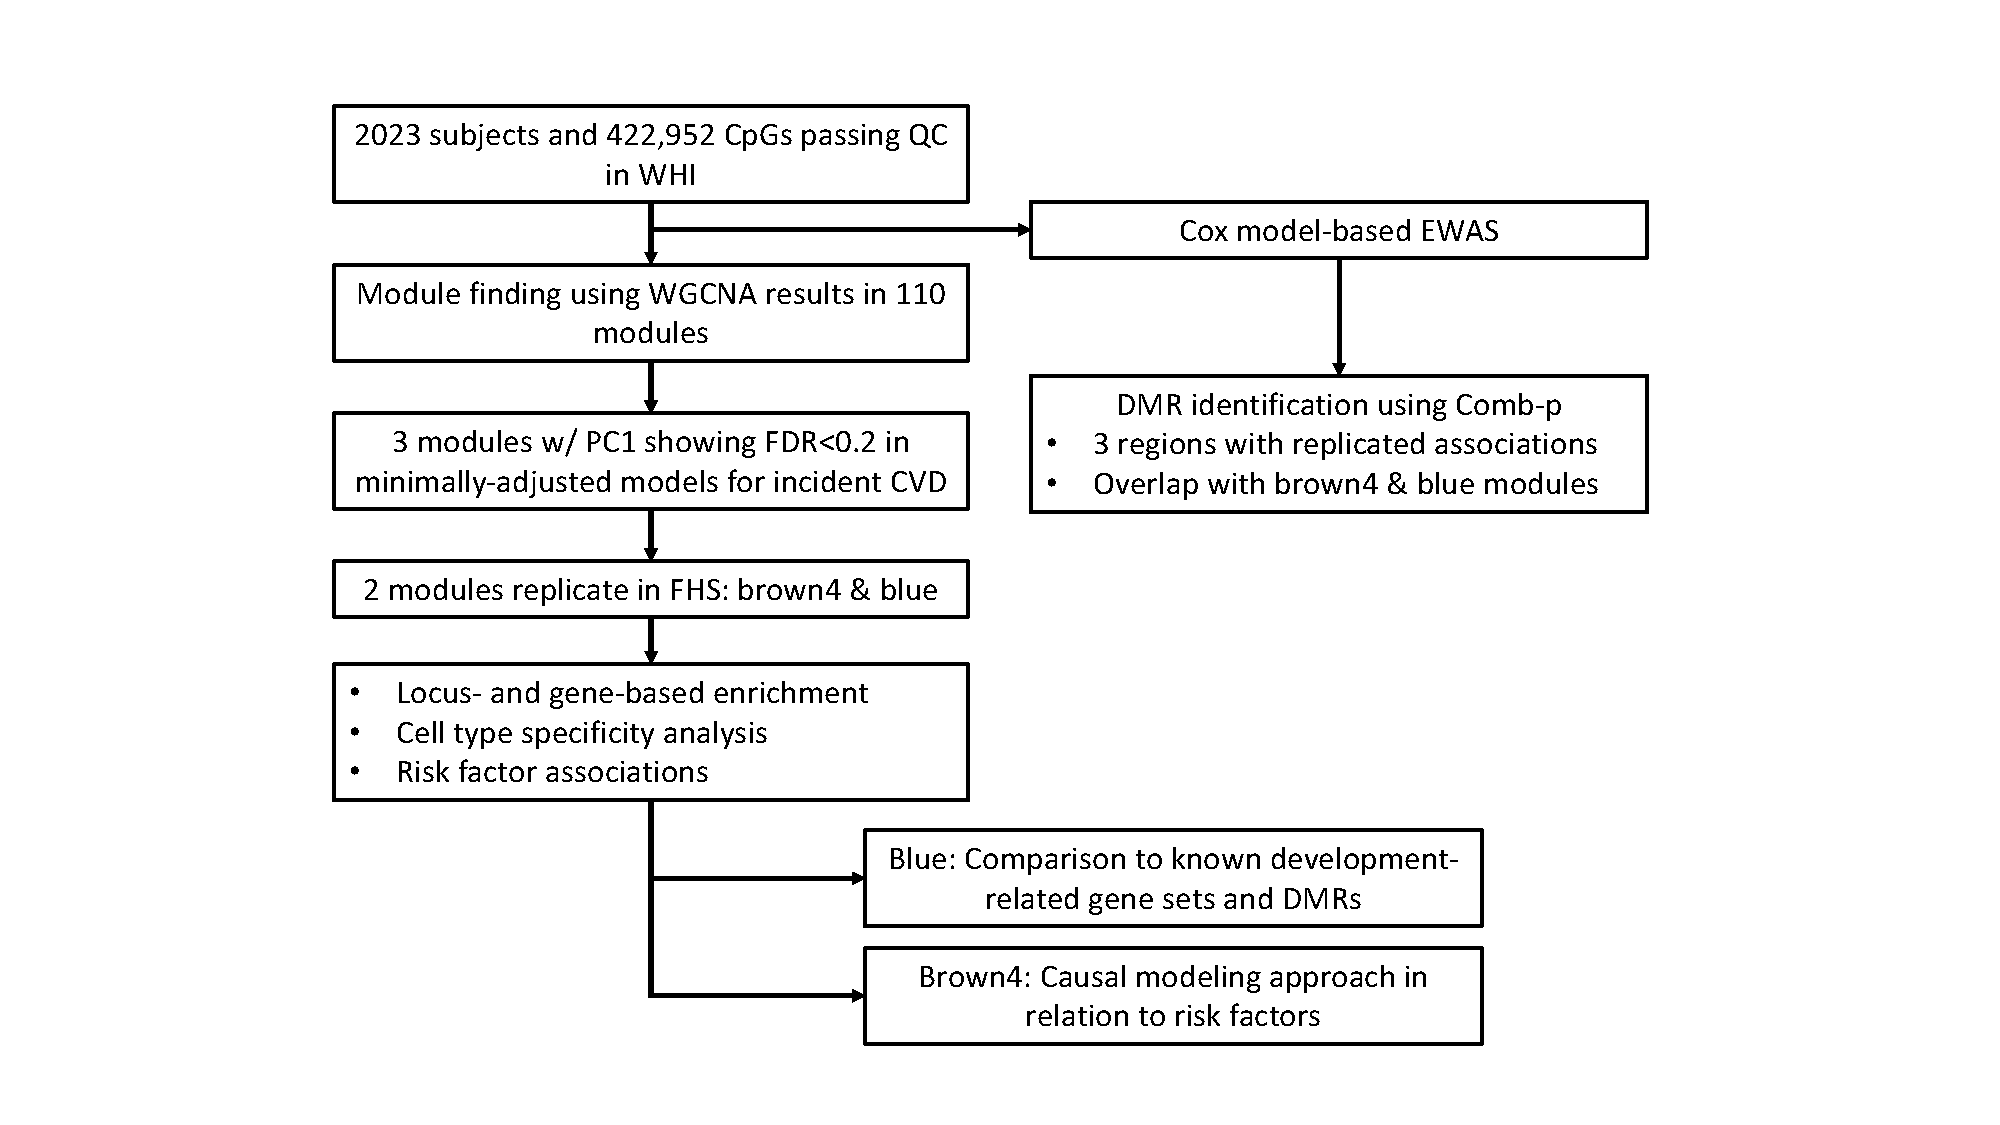
\includegraphics{workflow.pdf}
\caption{Computational workflow for MRS development and evaluation. The
initial MRS was trained in three cohorts with FHS-UM held out to
evaluate performance. The final MRS was then trained using all four
datasets and examined for biological significance, before testing for
prevalent MI discrimination in an independent cohort and assessment of
interactions with genetic and traditional risk scores.}
\end{figure}

\begin{figure}
\centering
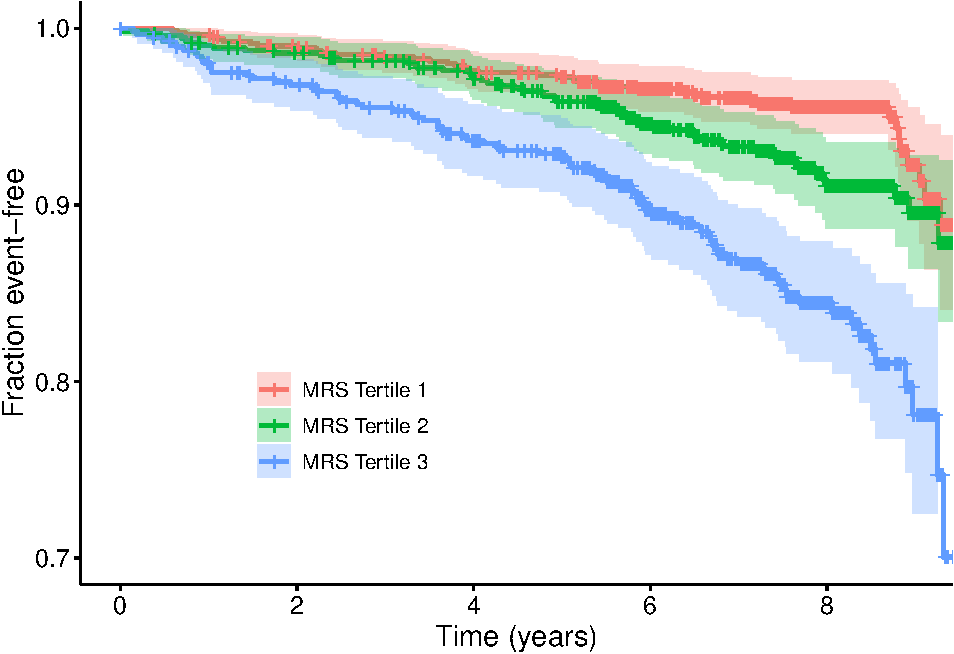
\includegraphics{figures/show-km-plot-1.pdf}
\caption{Kaplan-Meier survival curves in the held-out FHS-UM dataset.
Individual curves correspond to tertiles of the initial (3-dataset) MRS.
Vertical ticks correspond to censored observations, and colored bands
represent 95\% confidence intervals for tertile-specific survival
curves. X-axis is limited to the time span in which at least 50
uncensored observations remained for each tertile (3275 days).}
\end{figure}

\begin{figure}
\centering
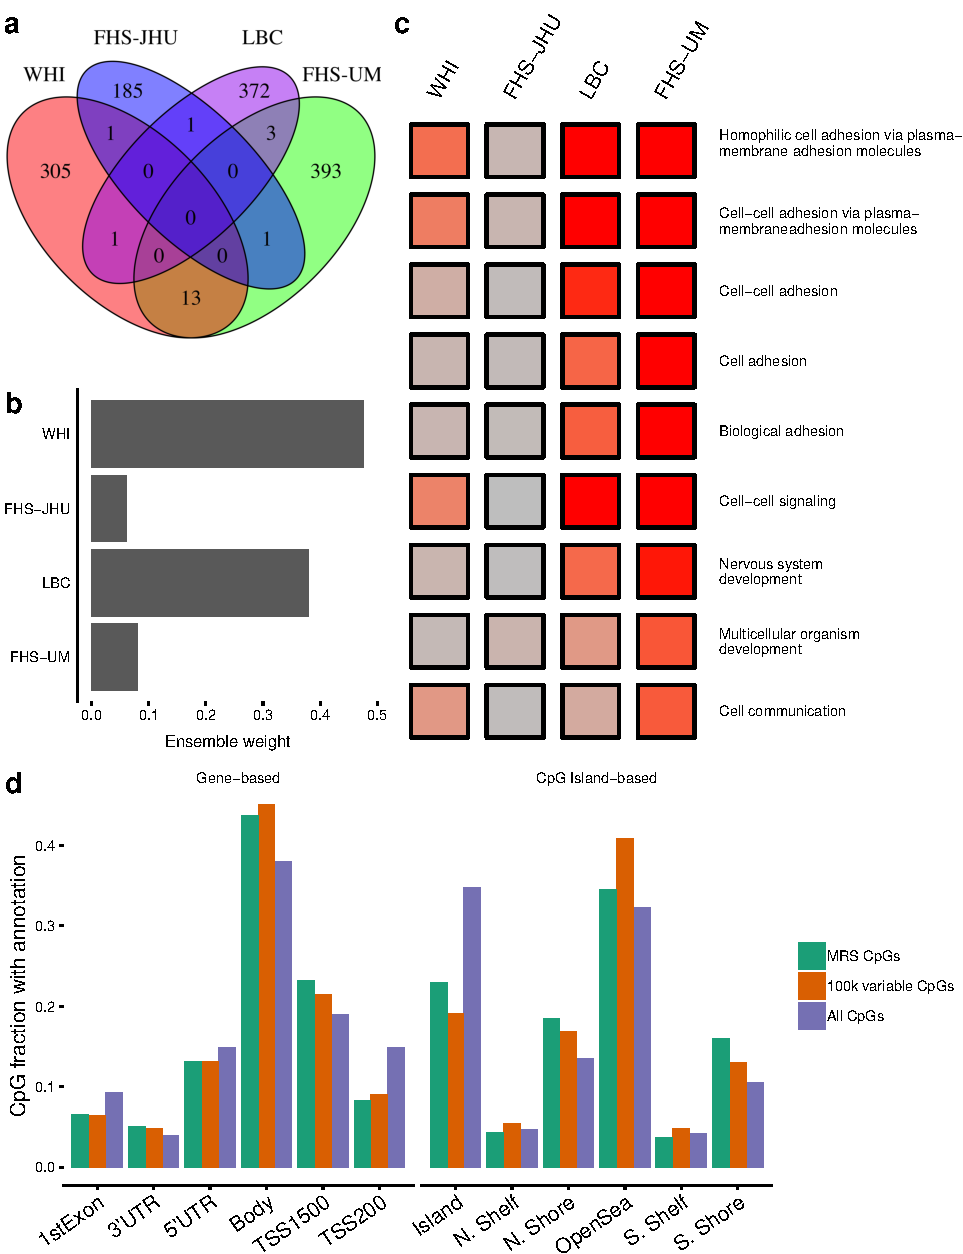
\includegraphics{figures/characterization-1.pdf}
\caption{Characterization of the final CSL model. a) Overlap of CpG
sites in the four individual predictors constituting the final model. b)
Study-specific weights for constructing the ensemble model (derived from
the ``stacking'' regression). c) Results from Gene Ontology-based
enrichment analysis using genes annotated to SSL component CpGs. All GO
terms with false discovery rate \textless{} 0.001 in any cohort are
shown, and colored according to -log(p-value) for enrichment in each
SSL. Values were cut at -log(p) = 20 for visualization purposes. d)
Proportion of CpGs in the full set of CSL CpGs (union of CpG sets in
each component SSL) compared to the 100,000 most variable CpGs (as used
in SSL model development) and the full set of available CpGs. Groupings
according to both gene-based and CpG island-based CpG annotations are
shown.}
\end{figure}

\begin{figure}
\centering
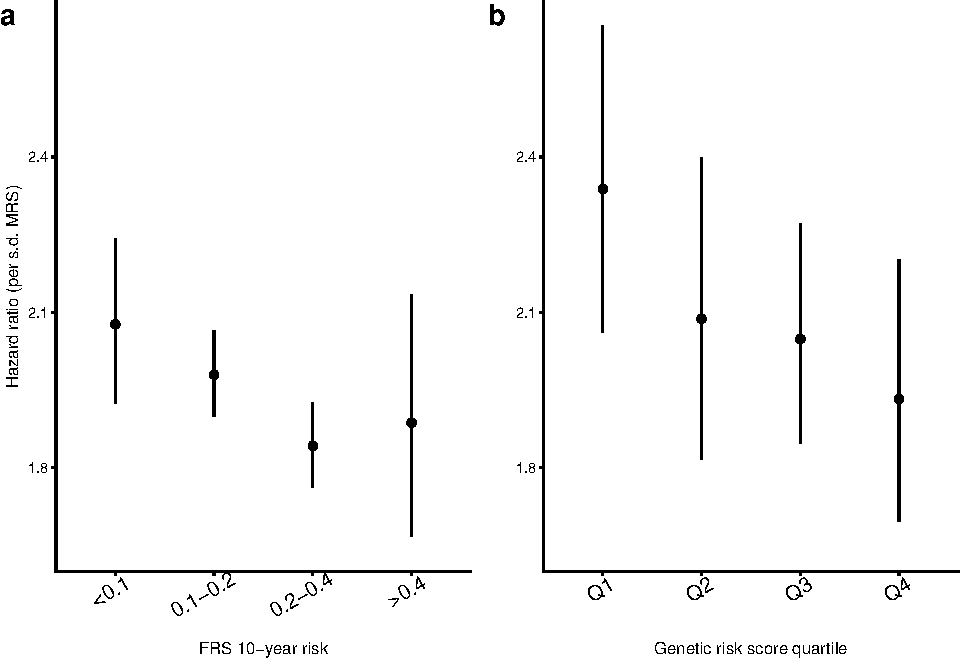
\includegraphics{figures/plot-aggregate-interactions-1.pdf}
\caption{Interactions of MRS with other biomarkers of CVD risk. a)
Hazard ratios for the MRS within subsets of 10-year generalized CVD risk
according to the Framingham Risk Score. b) Hazard ratios for the MRS
within quartiles of a genetic cardiovascular risk score (in white WHI
participants only). Hazard ratios are estimated using the final MRS,
which was trained using each of these datasets. Cox regressions included
stratum-specific baseline hazards and were adjusted for age, sex, and
estimated cell subtype fractions. Error bars represent standard errors
for the hazard ratio estimates.}
\end{figure}


\end{document}
